\documentclass[12pt,a4paper]{report}
\usepackage[utf8]{inputenc}
\usepackage[spanish]{babel}
\usepackage{amsmath}
\usepackage{amsfonts}
\usepackage{amssymb}
\usepackage{makeidx}
\usepackage{graphicx}
\usepackage{lmodern}
\usepackage{kpfonts}
\usepackage[left=2cm,right=2cm,top=2cm,bottom=2cm]{geometry}
\author{Eduardo Robles}
\title{Par de Rotacion y Cuaternios}
\begin{document}
\begin{center}

\includegraphics[scale=1]{logo.png}  
\end{center}
\begin{flushright}

Ingeniería mecatrónica 7-A\\
Cinemática de Robots \\
Eduardo Robles Vázquez\\
Fecha: 17/Septiembre/2019\\
\end{flushright}
\paragraph{PAR DE ROTACIÓN Y CUATERNIOS}

\subparagraph{Para manipular algún objeto con un robot se implica el movimiento de su extremo. De tal manera, para manipular una pieza es necesario conocer la ubicación y orientación con respecto a la base del robot de esta, por lo que se necesitan varias herramientas matemáticas para establecer relaciones espaciales entre distintos objetos que nos permitan saber la ubicación de uno respecto a otro.}


\subparagraph{Rotación }
\subparagraph{Rotación es el movimiento de cambio de orientación de un cuerpo o un sistema de referencia de forma que una línea (llamada eje de rotación) o un punto parece fijo. La rotación de un cuerpo se presenta mediante un operador que afecta un conjunto de puntos o vectores.}

\subparagraph{Par de rotación}
\begin{center}
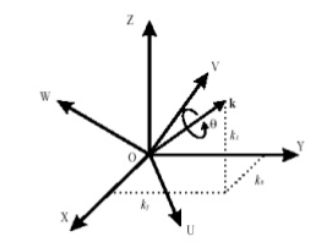
\includegraphics[scale=1]{2.png}  
\end{center}
\subparagraph{La aplicación que se le da a un par de rotación es que rote un vector p a un ángulo theta alrededor del vector unitario k, esto se realiza a través de la siguiente expresión:\\}
\begin{flushleft}
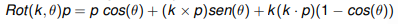
\includegraphics[scale=1]{1.png}  
\end{flushleft}
\subparagraph{\\
Cuaternios}
\subparagraph{
Los cuaternios son una extensión de los números reales, parecidos a los números complejos. Mientras que los números complejos son una extensión de los reales por la adición de la unidad imaginaria i, los cuaternios son una extensión generada de manera análoga añadiendo las unidades imaginarias: i, j y k a los números reales.\\
La utilización de los cuaterniones para representar una rotación ofrece una gran ventaja puesto que se puede evitar el problema de singularidad, esto quiere decir que exista alguna indeterminación al querer rotar con un cierto ángulo.\\}

\subparagraph{Matriz de transformación homogénea con cuaternios}

\subparagraph{El paso de cuaternios a la matriz de transformación homogénea, y viceversa, se pueden deducir fácilmente utilizando como representación auxiliar intermedia el eje y ángulo de rotación.\\
La matriz equivalente final es:}

\begin{center}
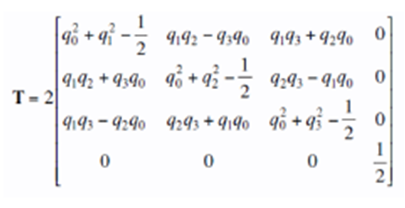
\includegraphics[scale=1]{22.png} 
\end{center}


\bibliography{biblio}
\bibliographystyle{plain}
\end{document}

